%%%%%%%%%%%%%%%%%%%%%%%%%%%%%%%%%%%%%%%%%%%%%%%%%%%%%%%%%%%
% EPFL report package, main thesis file
% Goal: provide formatting for theses and project reports
% Author: Mathias Payer <mathias.payer@epfl.ch>
%
% To avoid any implication, this template is released into the
% public domain / CC0, whatever is most convenient for the author
% using this template.
%
%%%%%%%%%%%%%%%%%%%%%%%%%%%%%%%%%%%%%%%%%%%%%%%%%%%%%%%%%%%
\documentclass[a4paper,11pt,oneside]{report}
% Options: MScThesis, BScThesis, MScProject, BScProject
\usepackage[BScThesis,lablogo]{EPFLreport}
\usepackage{xspace}

\title{Tooling and Analysis of the Scudo Allocator}
\author{Elias Valentin Boschung}
\supervisor{Mao Philipp Yuxiang}
\adviser{Prof. Dr. sc. ETH Mathias Payer}
%\coadviser{Second Adviser}
%\expert{The External Reviewer}

\newcommand{\sysname}{Scudo GEF Plugin\xspace}

\begin{document}
\maketitle{}
\makededication{}
\makeacks{}

\begin{abstract}
The \sysname{} tool enables inspection of the heap memory of an android app
which uses native C libraries.

While there is a lot of existent tooling to debug errors related to heap
memory in C code, it is only for the standard libc allocator. However,
Android uses its own allocator since Android 11, the scudo hardened
allocator. Since scudo uses its own structures and way to allocate memory,
those tools can not be used for debugging android C libraries.

In this project the goal was to analyze the way scudo allocates memory and
then write some tooling to debug it. The tool developed takes the form of
an extras plugin into the popular GEF plugin for GDB, which in turn is a
popular debugger for C programs.


The abstract serves as an executive summary of your project.
Your abstract should cover at least the following topics, 1–2 sentences for
each: what area you are in, the problem you focus on, why existing work is
insufficient, what the high-level intuition of your work is, maybe a neat
design or implementation decision, and key results of your evaluation.
\end{abstract}

\maketoc{}

%%%%%%%%%%%%%%%%%%%%%%
\chapter{Introduction}
%%%%%%%%%%%%%%%%%%%%%%

The introduction is a longer write-up that gently eases the reader into your
thesis~\cite{dinesh20oakland}. Use the first paragraph to discuss the setting.
In the second paragraph you can introduce the main challenge that you see.
The third paragraph lists why related work is insufficient.
The fourth and fifth paragraphs discuss your approach and why it is needed.
The sixth paragraph will introduce your thesis statement. Think how you can
distill the essence of your thesis into a single sentence.
The seventh paragraph will highlight some of your results
The eighth paragraph discusses your core contribution.

This section is usually 3–5 pages.

%%%%%%%%%%%%%%%%%%%%
\chapter{Background}
%%%%%%%%%%%%%%%%%%%%

Most standard android apps are written in Java, which is the main development
language for writing android apps. However, for more advanced uses there exists
support for including libraries written in standard C code, called native libraries
referring to the underlying structure of android which is actually a modified
version of Linux. These native libraries can be used together with Java code,
allowing C functions to be called from the java part of the code.

In C, the memory is divided into three big types that are handled differently.
There is the data segment, which contains the global and static variables that
are defined in a program, and the data segment can be further divided into the
initialized global and static variables, and the uninitialized or initialized to
zero global and static variables.
Then there is the stack, which is used for local variables in a function as well
as for arguments and some additional info about called functions. The size of
variables on the stack have to be fixed-size and the variable's lifetime is
limited to the scope of the function.
The third type of memory is the one important for this thesis, the heap memory.
The heap memory is the most flexible of the three types of memory, as it is not
limited to a specific lifetime like the stack and variables on the heap can be
resized. Heap memory can be allocated by the programmer by calling the \verb|malloc|
function, and unlike the stack or data segment, it has to be explicitly freed by
the programmer again, by calling \verb|free|. To resize a variable on the heap, the
\verb|realloc| function can be used. Since the variables have to be freed manually,
the programmer has full control over the lifetime of a variable on the heap, and
it can be used for variables that are needed outside the scope of a single
function. Furthermore, the heap has a virtually infinite amount of space, and is
generally also used for very big memory allocations. However, due to this big
flexibility, the handling of heap memory is also quite error-prone, by forgetting
to free allocated memory or allocating a chunk of the wrong size of the heap and
trying to access memory outside the allocated part.

Due to the ability to resize the heap variables and their flexible lifetime, the
heap cannot simply allocate contiguous chunks of memory in the order that variables
were allocated, as there would have to be a lot of moving when variables were
resized and there would be a lot of space lost when some chunks in the middle of
the heap were freed. Instead, there is a lot of bookkeeping done around which
chunks of memory are allocated, which are free and the heap allocator tries to
decide in a smart way which chunks to allocate when and where to get as much
performance as possible.

While the general concepts of these memory types are universal for the C language,
there are some differences in the concrete implementation, especially of the heap
allocator. While most Linux programs use the more standard libc malloc, which is
well documented and for which tooling exists to investigate the state of the heap,
android uses its own allocator since Android 11, which is called the scudo
hardened allocator.

Explain gdb, gef and gef extra plugins and how they come together/interact.


%%%%%%%%%%%%%%%%
\chapter{Scudo Internals}
%%%%%%%%%%%%%%%%

The scudo hardened allocator divides the heap allocations it is asked to do into
two big types of allocations, based on the size of the chunk to be allocated.
The smaller chunks are handled by the primary allocator inside scudo, which is
designed to optimize performance as much as possible by adapting to finer grained
size differences between these smaller chunks. All the big chunks are handled by
the secondary allocator, which is less optimized, since the most frequent chunks
are the small ones and thus the primary allocator has a bigger impact on performance
than the secondary allocator.

The chunks allocated by both the primary and the secondary allocator are prepended
by the same header, which holds some information about that chunk. This combined
header contains the ClassId, which identifies the class the chunk belongs to if
it was allocated by the primary allocator, with a ClassId of 0 meaning that the
chunk was allocated by the secondary allocator. The header also contains information
about the state of the chunk, which can be allocated, quarantined or available, as
well as the origin of the allocation, e.g., malloc or new, which can be used to
detect errors when the type of deallocation does not match the type of the
allocation. Furthermore, the header includes the size for the primary chunks or
the amount of unused bytes for the secondary chunks and an offset, which is the
distance from the beginning of the returned chunk to the beginning of the actual
backend allocation. Finally, the header contains a checksum, which is generated
using a cookie (a random number generated during the initialization of the
allocator), the heap address of the chunk, and the actual content of the header.
This checksum is used for guarding against programming errors as well as attackers,
and it is checked each time the header is loaded.

The primary allocator structures the heap into Classes (also named Regions), the
amount of which depend on the configuration. These classes are identified by a
ClassId, starting from 0. The first class, with ClassId 0, is however a special
class, that works differently than the other classes. The other classes have a
given size of the chunks that can be allocated in that class, which increases
with the ClassId, with the exact numbers depending again on the configuration.
So the chunk that is actually returned by the primary allocator might be bigger
than what was asked for, but this helps against having to do expensive bookkeeping
to avoid fragmentation inside the classes.
So when an allocation request is made to scudo, and it is small enough to fit into
one of the primary allocator regions, then the primary allocator first finds the
smallest class that still contains chunks big enough for the requested size. It
then checks in the cache associated to that class, to find a chunk that is already
available. However, if the cache is empty, meaning that there are no readily
available free chunks, the primary allocator tries to refill the cache with some
new chunks. For that purpose, it looks up the freelist of TransferBatches for the
given class, and if it is not empty it just takes all the chunks of the first
TransferBatch in the freelist and moves them to the cache of the class. One
TransferBatch holds a certain number of chunks defined by the configuration,
which is the same for all classes.
In case the freelist is out of TransferBatches, the allocator will allocate
some new TransferBatches to fill up the freelist. The amount of TransferBatches
allocated at one such time depends on the configuration, but it is typically
smaller the bigger the class gets, as one TransferBatch represents more actual
memory the bigger the class is. The allocator will also map more space for a
specific class if the amount of TransferBatches to be created does not fit into
the existing mapped space.
Since the transfer batches that are currently in one of the freelists need to
be stored somewhere as well, the first class with ClassId 0 is reserved for
this use. The allocations requested by the user will never directly use this
class, instead when a freelist for one of the classes needs to be refilled
with new TransferBatches, these are allocated in this first class, and they
are freed when they are moved to the cache of the class.

Additionally, while not yet present in the version of scudo shipped with Android
11, the latest scudo version includes a type that regroups multiple transfer
batches, into a BatchGroup. Instead of the freelist for a given class containing
a list of transfer batches, it now has a list of batch groups, which contain
a list of transfer batches each. The overall functionality of the allocator
doesn't change however, the change is just supposed to get even more performance
for the frequent allocations of the primary allocator.

The secondary allocator is a bit less sophisticated, since it does not need to
be able to do as many allocations and deallocations as the primary allocator,
and the optimizations of the primary allocator would not be that efficient for
the bigger and therefore generally more variable sizes the secondary allocator
has to handle. Instead, the secondary allocator just keeps a simple cache of
the previously freed chunks, and if there is no matching chunk in its cache
upon a request for a new allocation, it maps some new memory for that chunk.
For bookkeeping, the secondary allocator simply keeps a doubly linked list of
all chunks currently in use and keeps track of the details of each allocated
chunk in a special header that is prepended to the combined header.


%%%%%%%%%%%%%%%%%%%%%%%%
\chapter{Implementation}
%%%%%%%%%%%%%%%%%%%%%%%%

The structure of the gef-extras plugin is heavily inspired by the existing
structure of the tooling for the standard libc heap allocator used in most
Linux systems, which is included in the gef plugin for gdb. The scudo plugin
therefore offers multiple commands for the different structures present in
scudo. These commands take generally some address to a memory region, and
create an object by reading out the data from that memory address and parsing
it according to the predefined structure.

The most basic command is the \verb|scudo chunk| command, which given the address
of a chunk on the heap, reads the header in front of the chunk and displays
the info contained in it. The design of the output is the same as for the
standard libc heap commands included in gef, with the allocation state being
highlighted in color, as can be seen in \autoref{fig:ScudoChunkCommand}.
In the actual implementation, a chunk is represented as a class, and like in
gef, the different information is stored as properties of the class. Similarly,
the data is read from memory using the \verb|gef.memory.read| function, and then
structured as a type using the ctypes library to represent the different types
used in scudo. The \verb|str| method on the class is implemented to display a short
summary of the most essential info, while the \verb|psprint| method shows the
extended information display, as shown in \autoref{fig:ScudoChunkCommand}.

\begin{figure}[h!]
  \centering
  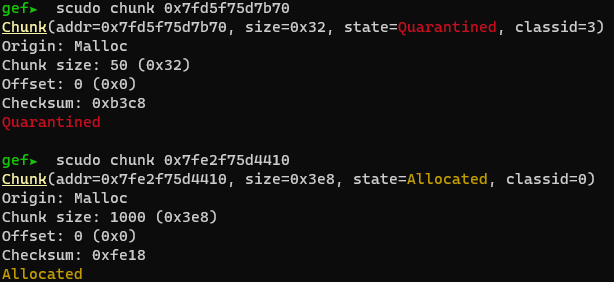
\includegraphics[width=\linewidth]{figures/ScudoChunkCommand.png}
  \caption{Example of the scudo chunk command in gef}
  \label{fig:ScudoChunkCommand}
\end{figure}

The next two commands concern the region info, with respectively the
\verb|scudo region| and \verb|scudo regions| commands. Both of work with the same
\verb|ScudoRegionInfo| class, which is defined like the scudo chunk with a ctypes
structure to represent the types in the scudo c code, and with properties for
all the information extracted. The one special thing about the region info
class is the padding, since the structure is padded to the scudo cache line
size for faster access. So the plugin first builds an unpadded version of the
ctypes structure, and then adds the required padding to get a multiple of the
scudo cache line size to the structure to get the final version.

The info included in the RegionInfo structure includes the list of transfer
batches for that region, the number of popped and pushed blocks, the amount
of memory mapped and allocated inside the region, the random state generated
for the region as well as information about the last release of blocks to
the operating system.

The data of this \verb|RegionInfo| structure is stored in an array, with an entry
for each of the regions/classes. The array is part of the primary allocator
class, and so the plugin finds it by using the offset from the \verb|Allocator|
symbol to get the first entry in the array.
The \verb|scudo regions| command then simply displays a list of short information
about each region, as seen in \autoref{fig:ScudoRegionsCommand}.

\begin{figure}[h!]
  \centering
  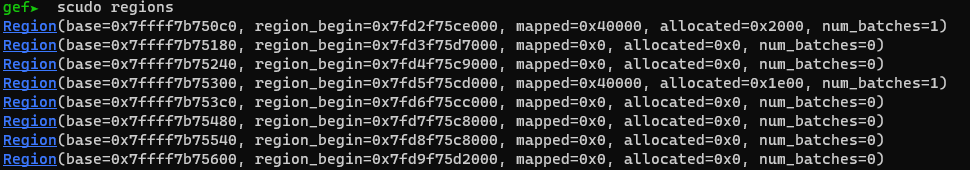
\includegraphics[width=\linewidth]{figures/ScudoRegionsCommand.png}
  \caption{Example of the scudo regions command in gef}
  \label{fig:ScudoRegionsCommand}
\end{figure}

The \verb|scudo region| command on the other hand displays more detailed information
about a specific region, which can be specified either by giving the address
to the RegionInfo structure, by giving the max allocation size of the region,
or by the index in the array, which corresponds to its ClassId. An example of
the display can be seen in \autoref{fig:ScudoRegionCommand}, which shows the
special region which holds the transfer batches.

\begin{figure}[h!]
  \centering
  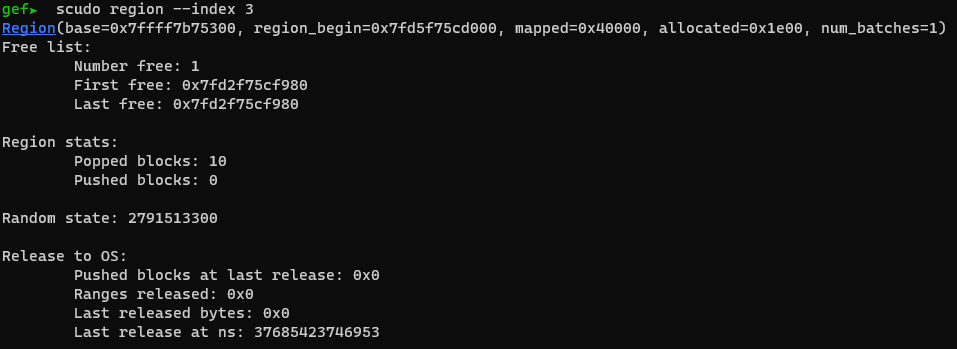
\includegraphics[width=\linewidth]{figures/ScudoRegionCommand.png}
  \caption{Example of the scudo region command in gef}
  \label{fig:ScudoRegionCommand}
\end{figure}

The next two commands concern the free list of the primary allocator, as they
display the information about the batch groups and the transfer batches. Both
of these commands are very simple, since both of them basically contain a list
of another structure. Also since there isn't one universal point where all of
them are stored, the commands need to be provided with the address of the
batch group or transfer batch to output.
Since the batch groups are a new addition, the command doesn't work on a real
Android 11 phone, however it works when using the standalone compiled version
from the llvm repository. It shows detailed information about the batch group,
including the address of the next batch group, since the batch groups form a
linked list, the number of pushed blocks, and the information about the doubly
linked list of transfer batches it contains. While this detailed view can be
seen in \autoref{fig:ScudoBatchGroupCommand}, when specifying a number as
argument with \verb|--number X|, it will instead display a short version for this
amount of batch groups in the linked list, with the first one being the one
specified by address.

\begin{figure}[h!]
  \centering
  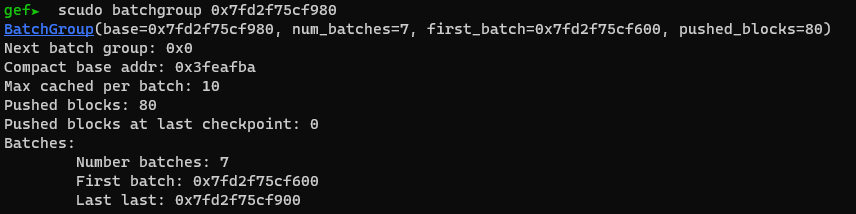
\includegraphics[width=\linewidth]{figures/ScudoBatchGroupCommand.png}
  \caption{Example of the scudo batch group command in gef}
  \label{fig:ScudoBatchGroupCommand}
\end{figure}

The \verb|scudo transferbatch| command simply outputs the addresses of every batch
it contains, as well the address of the next transfer batch, which can be seen
in \autoref{fig:ScudoTransferBatchCommand}. Since the transfer batches also
form a linked list similarly to the batch groups, the number argument can be
specified in the same way to get an overview of that number of transfer batches.

\begin{figure}[h!]
  \centering
  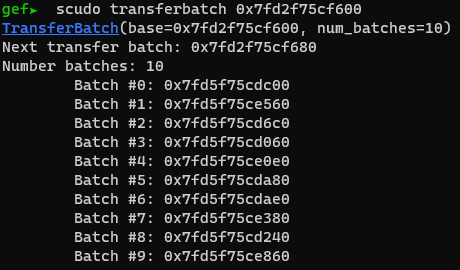
\includegraphics{figures/ScudoTransferBatchCommand.png}
  \caption{Example of the scudo transfer batch command in gef}
  \label{fig:ScudoTransferBatchCommand}
\end{figure}

The next command concerns the cache, which is actually the first place the
primary allocator tries to look for free chunks to allocate for the user.
While again the content of each per class structure is fairly simple with a
list of the chunks it contains and the maximal number of chunks it can contain,
there was a particular challenge about implementing this command, which was to
find the location of the actual array. Since scudo was designed for multi
threading, there actually exists a cache for each thread, and as such the per
class array of each thread is not simply stored at an offset from the Allocator
symbol. However, there luckily is a trick to find the different per class arrays
of the different threads, as the cache of each thread contains some statistics
about the allocated and free blocks in that cache. In order to have some global
statistics over all the different threads, scudo stores some global stats, that
include a linked list of all the local stats of the different threads. So in
order to get the address of the per class array of a thread, the plugin gets
the linked list of statistics from its offset to the Allocator symbol and then
follows the linked list the number of times to reach the statistics for the
correct thread. Since the statistics are stored right after the per class array
in the cache, the plugin then simply subtracts the size of the per class array
to get the address of the first entry in the class array.
For that reason the \verb|scudo perclass| command also takes two arguments, the first
being the thread id and the second being the class id, which uniquely define
the entry to get. If the ids are omitted a default value of 0 is taken. An
example of the output can be seen in \autoref{fig:ScudoPerClassCommand}.

\begin{figure}[h!]
  \centering
  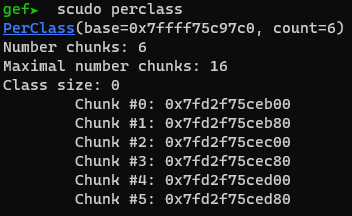
\includegraphics{figures/ScudoPerClassCommand.png}
  \caption{Example of the scudo per class command in gef}
  \label{fig:ScudoPerClassCommand}
\end{figure}

The last command is the only one concerning the secondary allocator specifically,
and it reads out the special header that is prepended to the normal chunk header
for any secondary chunk. The normal scudo chunk command still works for secondary
chunks as well though. The large block command gives information about the
commit and map base addresses and sizes, as well as the next and previous large
blocks in the linked list. The command can either be provided by an address
to read out the corresponding large block, or if the address is omitted it will
take the first block from the list of blocks in use. An example can be seen in
\autoref{fig:ScudoLargeBlockCommand}. A \verb|--number X| argument can optionally be
specified to get once again a list of short infos about that amount of large
blocks.

\begin{figure}[h!]
  \centering
  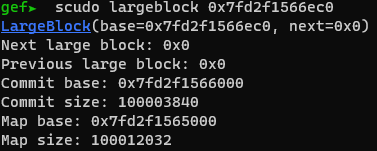
\includegraphics{figures/ScudoLargeBlockCommand.png}
  \caption{Example of the scudo large block command in gef}
  \label{fig:ScudoLargeBlockCommand}
\end{figure}

While the whole plugin is contained in a single file to follow the gef standard,
the organization with classes and using the ctypes structures allows for a
flexibility in adapting and evolving the plugin. As such it would be quite
easy to adapt the plugin for any minor changes in the scudo structure should
it evolve in the future, or adapted to support older versions of scudo, with
one such version already being implemented for the version of scudo that was
shipped with Android 11. The main changes for this older version of scudo
included that the batch groups did not exist yet, some minor reordering of
some fields in some of the structures, which also caused some of the offsets
from the Allocator symbol to be changed.


%%%%%%%%%%%%%%%%%%%%
\chapter{Evaluation}
%%%%%%%%%%%%%%%%%%%%

During the main development process the plugin was tested with the standalone
version of scudo compiled with debug symbols from the llvm repository. In
order to get the plugin loaded by gef, the folder containing the plugin file
needs to be specified as gef-extras plugin dir. The easiest way to do this
is to run \verb|gef config gef.extra_plugins_dir /path/to/plugin/dir|. In order
to use multiple different gef extra plugins that may be located at different
paths, multiple paths can be specified separated by semicolons. Also, the
configuration can be saved using \verb|gef save|, which will create a gef.rc file
that will be loaded in order to keep the settings between restarts of gdb.

Since the main development was done on the standalone version, the first step
to evaluate the plugin was to actually test it on a real android phone. The
test device was a Samsung Galaxy S10, which was already rooted using Magisk
and had gdb and gef installed using the Termux app. Access to the phones
console and copying of the plugin to the phone was done using adb. In order
to do the evaluation directly using WSL from a Windows workstation, the
usbipd driver was used to pass the phone connected using USB to WSL. Without
going into detail, the commands for attaching the phone to WSL to be entered
in an Administrator Command Prompt are the following, replacing X-X with the
busid shown in the first command for the android phone:
\begin{verbatim}
usbipd wsl list
usbipd wsl attach --busid X-X
\end{verbatim}

While the plugin installation and loading worked without problem on the phone, it
rapidly became evident that the plugin did not work as intended and instead
returned some random looking numbers for most commands. So after some
investigation, it was discovered that the scudo version shipped with Android
11, which was installed on the testing device, differed in multiple points
from the most recent version on the llvm repository. The plugin was therefore
copied and adapted into a version for Android 11, which notably does not
contain the batch groups, as well as differing in some minor changes in
different structures.



Give some examples of the crashes analyzed, how the commands of the plugin
can be used to figure out what is happening.

In the evaluation you convince the reader that your design works as intended.
Describe the evaluation setup, the designed experiments, and how the
experiments showcase the individual points you want to prove.

This section is usually 5–10 pages.


%%%%%%%%%%%%%%%%%%%%%%
\chapter{Related Work}
%%%%%%%%%%%%%%%%%%%%%%

Mention some of the links as provided for the beginning of the project.

The related work section covers closely related work. Here you can highlight
the related work, how it solved the problem, and why it solved a different
problem. Do not play down the importance of related work, all of these
systems have been published and evaluated! Say what is different and how
you overcome some of the weaknesses of related work by discussing the 
trade-offs. Stay positive!

This section is usually 3–5 pages.


%%%%%%%%%%%%%%%%%%%%
\chapter{Conclusion}
%%%%%%%%%%%%%%%%%%%%

In the conclusion you repeat the main result and finalize the discussion of
your project. Mention the core results and why as well as how your system
advances the status quo.

\cleardoublepage{}
\phantomsection{}
\addcontentsline{toc}{chapter}{Bibliography}
\printbibliography{}

% Appendices are optional
% \appendix
% %%%%%%%%%%%%%%%%%%%%%%%%%%%%%%%%%%%%%%
% \chapter{How to make a transmogrifier}
% %%%%%%%%%%%%%%%%%%%%%%%%%%%%%%%%%%%%%%
%
% In case you ever need an (optional) appendix.
%
% You need the following items:
% \begin{itemize}
% \item A box
% \item Crayons
% \item A self-aware 5-year old
% \end{itemize}

\end{document}
